% https://github.com/martinhelso/MathDept


\documentclass[UKenglish]{beamer}


\usetheme[NoLogo]{MathDept}


\usepackage[utf8]{inputenx} % For æ, ø, å
\usepackage{babel}          % Automatic translations
\usepackage{csquotes}       % Quotation marks
\usepackage{microtype}      % Improved typography
\usepackage{amssymb}        % Mathematical symbols
\usepackage{mathtools}      % Mathematical symbols
\usepackage{comment}        % Comment out multiple lines
\usepackage[absolute, overlay]{textpos} % Arbitrary placement
\setlength{\TPHorizModule}{\paperwidth} % Textpos units
\setlength{\TPVertModule}{\paperheight} % Textpos units
\usepackage{tikz}
\usetikzlibrary{snakes}
\usetikzlibrary{calc}
\usetikzlibrary{intersections}
\usetikzlibrary{decorations.markings}
\usetikzlibrary{decorations.pathreplacing,calligraphy}

\usetikzlibrary{overlay-beamer-styles}  % Overlay effects for TikZ

% Added by me 
\newcommand{\E}{\mathbb{E}}  % expectation
\newcommand{\F}{\mathcal{F}} % Filtration 

\newcommand{\R}{\mathbb{R}}  % Real numbers

% Limits
\usepackage{amsmath}

% Indicator function 
\usepackage{bbm}

% Midrule lines in tabels:
\usepackage{booktabs}





\author{Andreas Slåttelid}
\title{MSc Thesis}
\subtitle{Advancements in Risk-Free Reference Rates and ESG-linked interest rate swaps}



\begin{document}


%\section{Overview}


% Use
%
%     \begin{frame}[allowframebreaks]{Title}
%
% if the TOC does not fit one frame.
\begin{frame}{Table of contents}
    \tableofcontents[currentsection]
\end{frame}


\section{Interest rate theory}
\SectionPage
\subsection{Framework}

\begin{frame}{Framework}
\begin{itemize}
    \item $(\Omega, \F, \mathbb{F}, P)$ probability space.  
    \item $\mathbb{F} = \{\F_{t}, t \in [0,T]\}$, right-continous and augmented, $T$ a fixed time horizon. 
    \item $W = \{W(t), t\in [0,T]\}$ a one-dimensional Brownian Motion. 
    \item $\mathcal{E} = \{\mathcal{E}_{t}(\gamma \bullet W), t \in [0,T]\}$ where: 
    \begin{align*}
     \mathcal{E}_{t}(\gamma \bullet W) := \exp\left(
     \int_{0}^{t}\gamma(s)dW(s) -\frac{1}{2}\int_{0}^{t}\gamma^{2}(s)ds
     \right)   
    \end{align*}
    \item We assume that the Novikov condition holds:
    \begin{align*}
     \E\left[
     \exp\left(
     \frac{1}{2}\int_{0}^{T}|\gamma(s)|^{2}ds
     \right)
     \right] < \infty   
    \end{align*}
\end{itemize}
\end{frame}


\begin{frame}{Framework}
\begin{itemize}
    \item This means that: 
    \begin{align*}
    \frac{dQ}{dP}\bigg{|}_{\F_{T}} := \mathcal{E}_{T}(\gamma \bullet W)   
    \end{align*}
    Is well-defined, furthermore $\mathcal{E}$ is a martingale, and from Girsanov's theorem, we have that: $W^{Q} = \{W^{Q}(t), t\in [0,T]\} $ is a $Q$-Brownian Motion defined on $(\Omega, \F, Q)$
\end{itemize} 
\end{frame}

\begin{frame}{Financial market}
\begin{itemize}
    \item $r = \{r(t), t\in [0,T]\}$ short-rate process such that $\int_{0}^{t}r(s)ds$ is well-defined, with $Q$-dynamics given by: 
    \begin{align*}
    dr(t) &= b(t,r(t))dt + \sigma(t,r(t))dW^{Q}(t)  \\
    r(0) &= r_{0} \in \R
    \end{align*}
    $b(t,x)$ and $\sigma(t,x)$ are assumed to be so 
    that the above SDE possess a unique and strong solution. 
    \item $B = \{B(t), t\in [0,T]\}$ the money market account, defined as: 
    \begin{align*}
        B(t) &= \exp\left(
        \int_{0}^{t}r(s)ds
        \right)
    \end{align*}
    \item $P(s,t)$ market value at time $s$ for a zero-coupon bond (ZCB) maturing at time $t,\; 0\leq s\leq t \leq T$. Guarantees its holder one unit of account at maturity. 
\end{itemize}
\end{frame}

\begin{frame}{Term Structure}
    \begin{itemize}
        \item A collection $\{P(s,t), 0\leq s \leq t \leq T\}$,  is called a term structure.
        \item Relationship between the short-rate and the ZCB:
        \begin{align*}
        P(t,T) &= \E_{Q}\left[
        \exp\left(
        -\int_{t}^{T}r(s)ds
        \right)\bigg{|}\F_{t}
        \right]    
        \end{align*}
    \item Assume that there exists a smooth function: 
    \begin{align*}
        g:\{(s,t)\in [0,T]\times [0,T]: s\leq t\}\times \R \to \R
    \end{align*}
    such that $P(s,t) = g(s,t,r(s))$. If: 
    \begin{align*}
    g(t,s,r(s)) &= \exp\left(
    -A(s,t)-B(s,t)r(s)
    \right)    
    \end{align*}
    we say that we have an affine term structure (ATS). ($A,B$ smooth $C^{1}$-functions).  
    \end{itemize}
\end{frame}

\begin{frame}{Interest rate swap}

An Interest Rate Swap (IRS) is a financial agreement between parties to exchange interest payments on a specific nominal $N$. The idea is to exchange floating and fixed rates.

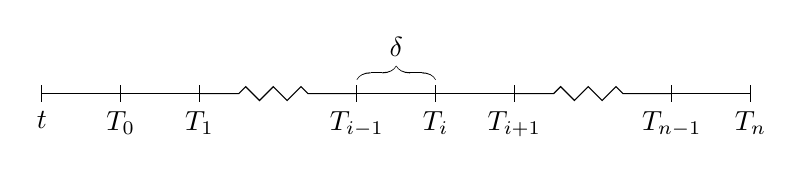
\begin{tikzpicture}[snake=zigzag, line before snake = 5mm, line after snake = 5mm]
    % draw horizontal line   
    \draw (0,0) -- (2,0);
    \draw[snake] (2,0) -- (4,0);
    \draw (4,0) -- (6,0);
    \draw[snake] (6,0) -- (8,0);
    \draw (8,0) -- (9,0);
    % Calligraphic brace
    \draw [
    decorate, 
    decoration = {calligraphic brace,
                  raise=5pt,
                  amplitude=5pt,
                  aspect=0.50}] (4,0) --  (5,0)
                  node[pos=0.50, above =1 0pt,black]{$\delta$};

    % draw vertical lines
    \foreach \x in {0,1,2,4,5,6,8,9}
      \draw (\x cm,3pt) -- (\x cm,-3pt);

    % draw nodes
    \draw (0,0) node[below=3pt] {$ t $} node[above=3pt] {$   $};
    \draw (1,0) node[below=3pt] {$ T_{0} $} node[above=3pt] {$  $};
    \draw (2,0) node[below=3pt] {$ T_{1} $} node[above=3pt] {$  $};
    \draw (3,0) node[below=3pt] {$  $} node[above=3pt] {$  $};
    \draw (4,0) node[below=3pt] {$ T_{i-1} $} node[above=3pt] {$  $};
    \draw (5,0) node[below=3pt] {$ T_{i} $} node[above=3pt] {$   $};
    \draw (6,0) node[below=3pt] {$ T_{i+1} $} node[above=3pt] {$  $};
    \draw (8,0) node[below=3pt] {$ T_{n-1} $} node[above=3pt] {$  $};
    \draw (9,0) node[below=3pt] {$ T_{n} $} node[above=3pt] {$  $};
  \end{tikzpicture}

\begin{itemize}
    \item $N$ nominal value. 
    \item $0 < T_{0} < T_{1} < \dots < T_{n}$ sequence of future dates. 
    \item $\delta := T_{i} - T_{i-1}$ fixed leg between payments. 
    \item $\kappa$ fixed rate 
    \item $F(T_{i-1}, T_{i})$ floating rate over $[T_{i-1}, T_{i}]$. 
\end{itemize}

The floating rate will reset at $T_{0}, \dots, T_{n-1}$ and the fixed rate will be paid at $T_{1}, \dots, T_{n}$. 
 
\end{frame}

\subsection{Interest rate swap}

\begin{frame}{Interest rate swap}
Perspective from payer IRS, at each instance $T_{i} , i = 1, \dots n$: 
\begin{itemize}
    \item Pay $\kappa \delta N$ (-)
    \item Receive $F(T_{i-1}, T_{i})\delta N$ (+)
\end{itemize}

Time-$t$ value $t\leq T_{0}$ of total cashflow: 

\begin{align*}
\pi(t) &= N[P(t,T_{0})- P(t,T_{n})] - \kappa \delta N \sum_{i=1}^{n}P(t,T_{i})     
\end{align*}

Now, the fixed swap-rate $\kappa = R_{Swap}(t)$, should be chosen such that $\pi(t) = 0$, namely: 
\begin{align*}
\kappa &= \frac{
P(t,T_{0}) - P(t,T_{n})
}{
\delta \sum_{i=1}^{n}P(t,T_{i})
}    
\end{align*}

\end{frame}


\section{RFR's/SOFR}
\SectionPage

\subsection{LIBOR scandal}
\begin{frame}{LIBOR scandal}
\begin{itemize}
    \item LIBOR: Interbank rate provided by panel banks for multiple tenors. 
    \item 2012: International-investigation. Collusion and rate-rigging: Barclays, UBS, Royal Bank of Scotland + others. 
    \item Reliability, transparency and trust were needed, hence the demand for new alternative reference rates.
    \item Solution: US: Secured Overnight Financing Rate (SOFR), UK: Sterling Overnight Index Average (SONIA). Similar alternatives exist in other countries as well.  
\end{itemize}
\end{frame}

\subsection{SOFR}
\begin{frame}{SOFR}
\begin{itemize}
    \item SOFR: overnight rate, developed by ARRC and managed by New York Fed.
    \item Based upon overnight Repo-market, backed up by US treasury securities. 
    \item Volume-weighted median. 
\end{itemize} 

\begin{definition}[Discrete overnight, backward-looking avarage]
\begin{align*}
R_{d_{i}}(T_{i}) &= \frac{1}{d_{i}}\left(
\frac{1}{P(T_{i}, T_{i}+d_{i})} - 1
\right) \\ 
R^{B}(S,T) &= \frac{1}{T-S}\left(
\prod_{i=1}^{N}[1+d_{i}R_{d_{i}}(T_{i})] - 1
\right)
\end{align*}
$d_{i}$: day count fraction. 

\end{definition}

\end{frame}


\begin{frame}{SOFR}
\begin{figure}[htp]
    \centering
    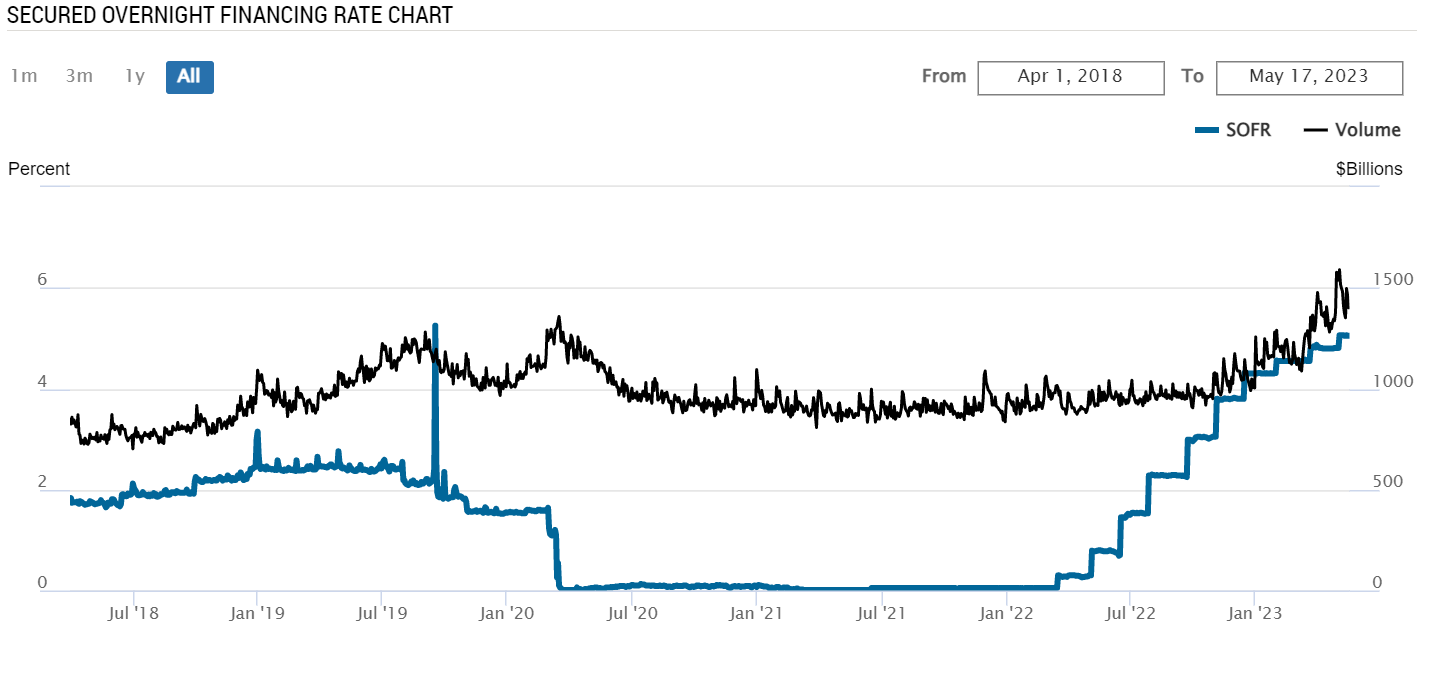
\includegraphics[height = 6cm, width=12cm]{SOFR/SOFR_Repo.PNG}
    \caption{O/N-SOFR and Repo volume}
    %\label{fig: ON_1M_3M_SOFR}
\end{figure}
Source: \url{https://www.newyorkfed.org/markets/reference-rates/sofr}
\end{frame}

\begin{frame}{SOFR-futures}
\begin{itemize}
    \item SOFR, overnight rate, outlook: 24 hours. 
    \item CME (Chicago Mercantile Exchange), publish term SOFR. 
    \item tenors: 1M, 3M, 6M and 12M. 
    \item Inferred from the futures market. 
\end{itemize}


\begin{definition}[1M- and 3M-SOFR futures]
\begin{align*}
f^{1M}(t,S,T) &= \frac{1}{T-S}\E_{Q}\left[
\int_{S}^{T}r(s)ds\bigg{|}\F_{t}
\right]\;\;(\text{arithmetic}) \\ 
f^{3M}(t,S,T) &= \frac{1}{T-S}\left(
\E_{Q}\left[
e^{\int_{S}^{T}r(s)ds}\bigg{|}\F_{t}
\right] - 1
\right)\;(\text{geometric})
\end{align*}    
\end{definition}
\end{frame}

\subsection{Hedging 3M-arithmetic rate}

\begin{frame}{Hedging 3M-arithmetic rate}
\begin{itemize}
    \item Loan of 30 Millon dollars over a 3M-period. 
    \item 3M-arithmetic floating-rate $X^{3M_{A}}(S,T)$ is to be paid, over this period. 
    \begin{align*}
    X^{3M_{A}}(S,T) &= \frac{1}{T-S}\int_{S}^{T}r(u)du
    \end{align*}
    \item Available products in market: 1M-SOFR futures and 3M-SOFR futures. 
    \item Short-rate $r = \{r(t), t\in [0,T]\}$ follows Vasicek-dynamics: 
    \begin{align*}
     dr(t) &= \alpha[m-r(t)]dt + \sigma dW^{Q}(t)   
    \end{align*}
\end{itemize}
\end{frame} 


\begin{frame}{Hedge 1}
\begin{itemize}
    \item Hedge possibility number one: using the available 3M-SOFR futures: 
\begin{align*}
\underset{a_{t}\in \R}{\arg\min}
&\E_{Q}\left[
\left(
X^{3M_{A}}(S,T)-a_{t}f^{3M}(t,S,T)
\right)^{2}
\bigg{|}\F_{t}
\right] \\ 
&= \frac{
\int_{S}^{T}\E_{Q}[r(u)|\F_{t}]du
}{
(T-S)f^{3M}(t,S,T)
}      
\end{align*}

\end{itemize}
\end{frame}


\begin{frame}{Hedge 1}
\begin{itemize}
    \item $r$ ATS: $dr(t) = [b(t) + \beta(t)r(t)]dt + \sqrt{a(t) + \alpha(t)r(t)}dW^{Q}(t)$ 
\begin{align*}
\underset{a_{t}\in \R}{\arg\min}
&\E_{Q}\left[
\left(
X^{3M_{A}}(S,T)-a_{t}f^{3M}(t,S,T)
\right)^{2}
\bigg{|}\F_{t}
\right] \\ 
&= 
\frac{
r(t)(T-S)
+ \int_{S}^{T}\int_{t}^{u}b(s)dsdu 
+ \int_{S}^{T}\int_{t}^{u}\beta(s)g(s)dsdu
}{
(T-S)f^{3M}(t,S,T)
}
\end{align*}

Where: 
\begin{align*}
g(s) &= \exp\left(
\int_{t}^{s}\beta(v)dv
\right)
\left(
\int_{t}^{s}e^{-\int_{t}^{w}\beta(v)dv}b(w)dw + \E_{Q}[r(t)]
\right) 
\end{align*}

\end{itemize}
\end{frame}


\begin{frame}{Hedge 2}
\begin{itemize}
    \item Hedge possibility number two: use available 1M-SOFR futures: 
\begin{align*}
&Y(a_{t}, b_{t}, c_{t}) \\
&:= 
a_{t}f^{1M}(t,S,T_{1M}) + 
b_{t}f^{1M}(t,T_{1M}, T_{2M}) + 
c_{t}f^{1M}(t,T_{2M}, T)
\end{align*}    
The hedge looks like this: 
\begin{align*}
\underset{(a_{t}, b_{t}, c_{t})\in \R^{3}}{\arg\min}
&\E_{Q}\left[
\left(
X^{3M_{A}}(S,T)-Y(a_{t}, b_{t}, c_{t})
\right)^{2}
\bigg{|}\F_{t}
\right]    
\end{align*}
\end{itemize}
\end{frame}

\begin{frame}{Hedge 2}

\begin{itemize}
    \item $\mathbf{x}_{t} = (a_{t}, b_{t}, c_{t})$, weightings in 1M-SOFR future rates.  
    \item SOFR-future rates:
    \begin{align*}
    \left(
    f^{1M}(t,S,T_{1M}), f^{1M}(t,T_{1M}, T_{2M}), f^{1M}(t,T_{2M}, T)
    \right)
    &= (\alpha_{t}, \beta_{t}, \gamma_{t})
    \end{align*}
    \item If $\det(M)\neq 0$, where:
    \begin{align*}
    M &= 
    \begin{bmatrix}
    \alpha_{t}^{2} & \alpha_{t}\beta_{t} &  \alpha_{t}\gamma_{t} \\ 
    \beta_{t}^{2} & \alpha_{t}\beta_{t} &   \beta_{t}\gamma_{t} \\ 
    \gamma_{t}^{2} & \alpha_{t}\gamma_{t} &     \beta_{t}\gamma_{t}
    \end{bmatrix}
    \end{align*}
    \item Optimal weight $\hat{\mathbf{x}}_{t}$ given by: 
    \begin{align*}
    \hat{\mathbf{x}}_{t} &= M^{-1}\E_{Q}\left[
    X^{3M_{A}}(S,T)\bigg{|}\F_{t}
    \right]
    \begin{bmatrix}
    \alpha_{t} \\ 
    \beta_{t} \\ 
    \gamma_{t} 
    \end{bmatrix}
    \end{align*}
\end{itemize}

\end{frame}

\begin{frame}{Numerical example}
\begin{itemize}
    \item Vasicek parameters: 
    \begin{align*}
    \alpha = 0.25, \; m = 0.035, \sigma = 0.02, r_{0} = 0.0425  
    \end{align*} 
    \item SOFR futures rates: 
    \begin{align*}
    f^{3M}(0,S,T) &= 0.0423
    \;\;\text{and}\;\;
    \begin{bmatrix}
    \alpha_{0} \\ 
    \beta_{0} \\ 
    \gamma_{0} 
    \end{bmatrix}
    =
    \begin{bmatrix}
    0.0423 \\ 
    0.0421 \\ 
    0.0420 
    \end{bmatrix}
    \end{align*}
    \item $\hat{a}_{t}^{3M}$: optimal weiging in 3M-SOFR futures rates. 
    \item $(\hat{a}_{t}^{1M}, \hat{b}_{t}^{1M}, \hat{c}_{t}^{1M})$: optimal weights in 1M-SOFR futures rates. 
    \item We choose to look at the following to benchmark the hedges:
    \begin{align*}
    ER_{1}(t) :&= X^{3M_{A}}(S,T) - \hat{a}_{t}^{3M}f^{3M}(t,S,T) \\ 
    ER_{2}(t) :&= X^{3M_{A}}(S,T) - Y(\hat{a}_{t}^{1M}, \hat{b}_{t}^{1M}, \hat{c}_{t}^{1M})
    \end{align*}    
\end{itemize}
    
\end{frame}


\begin{frame}{Numerical example}
\begin{itemize}
    \item 1 Million simulations:
\end{itemize}

\begin{figure}[htp]
    \centering
    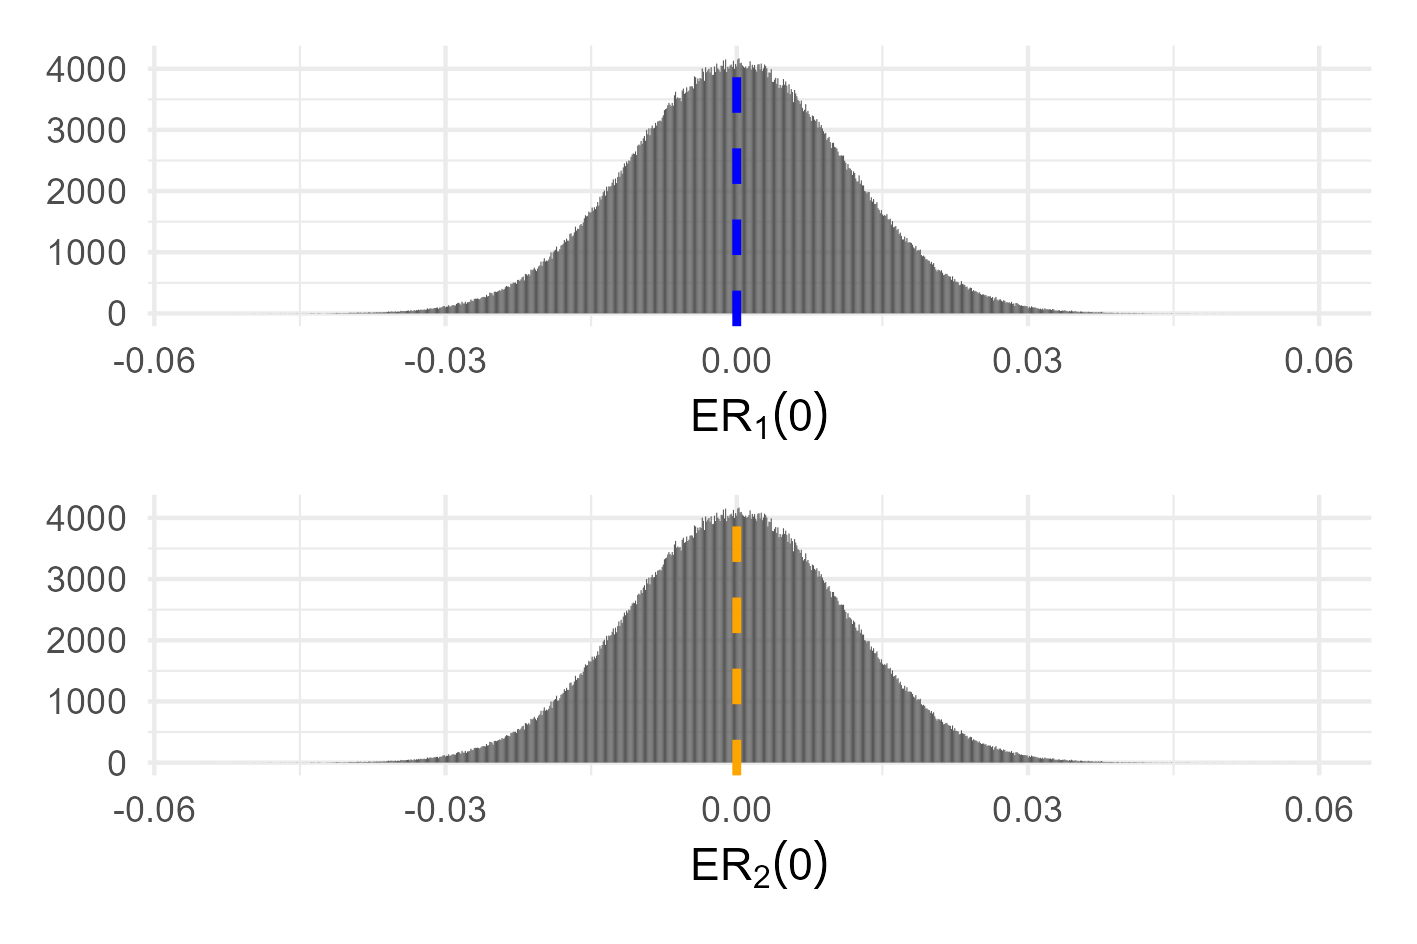
\includegraphics[width=9.5cm]{SOFR/SOFR_error_plt.png}
    \caption{$ER_{1}(0)$ and $ER_{2}(0)$}
    \label{fig: SOFR_error_plt}
\end{figure}

    
\end{frame}


\section{ESG}
\SectionPage

\subsection{Motivation}
\begin{frame}{ESG}
\begin{itemize}
    \item ESG: Environmental, Social and Governance
    \item EU: taxonomy, carbon neutral by 2050.  
    \item Partial Solution: Sustainable Finance,
          ESG-linked interest rate swap. 
    \item ISDA: SBM Offshore and ING, the world's first sustainability improvement derivative
    \cite{ISDA_2021}. 
    \item SBM pays fixed and receives floating. 
    \item ESG-part: If SBM meets certain ESG criteria, a 5-10 bp discount is applied to the fixed rate. Conversely, a penalty of 5-10 bp is added.  
\end{itemize}
\end{frame}


\subsection{ESG fixed rate}

\begin{frame}{ESG fixed rate}
Consider the following setup: 
\begin{itemize}
    \item $d$: basis points added or subtracted to fixed-rate $\kappa$. 
    \item $\{A_{i}\}_{i=1}^{n}$ sequence of events, where: 
    $A_{i} = \{X_{T_{i}} \leq C_{T_{i}}^{ESG}\}$
    i.e. the sequence of events measuring if the ESG-risk score at time $T_{i}$: $X_{T_{i}}$, is below the ESG-criteria $C_{T_{i}}$ or not. 
\end{itemize}

\begin{definition}[ESG-fixed rate process]
Let $K^{ESG} = (K_{i}^{ESG}(\omega))_{i=1}^{n}$ 
denote the ESG fixed rate process, we define it recursively as: 

\begin{align*}
K_{i}^{ESG}(\omega) &= (K_{i-1}^{ESG}(\omega)-d)\mathbbm{1}_{A_{i}}(\omega)
+ (K_{i-1}^{ESG}(\omega)+d)\mathbbm{1}_{A_{i}^{C}}(\omega), \;\; i\geq 2
\end{align*}

Where:
\begin{align*}
K_{1}^{ESG}(\omega) &= (\kappa - d)\mathbbm{1}_{A_{1}}(\omega)
+ (\kappa + d)\mathbbm{1}_{A_{1}^{C}}(\omega)    
\end{align*}
\end{definition}

\end{frame}

\begin{frame}{ESG fixed rate}
\begin{figure}[htp]
    \centering
    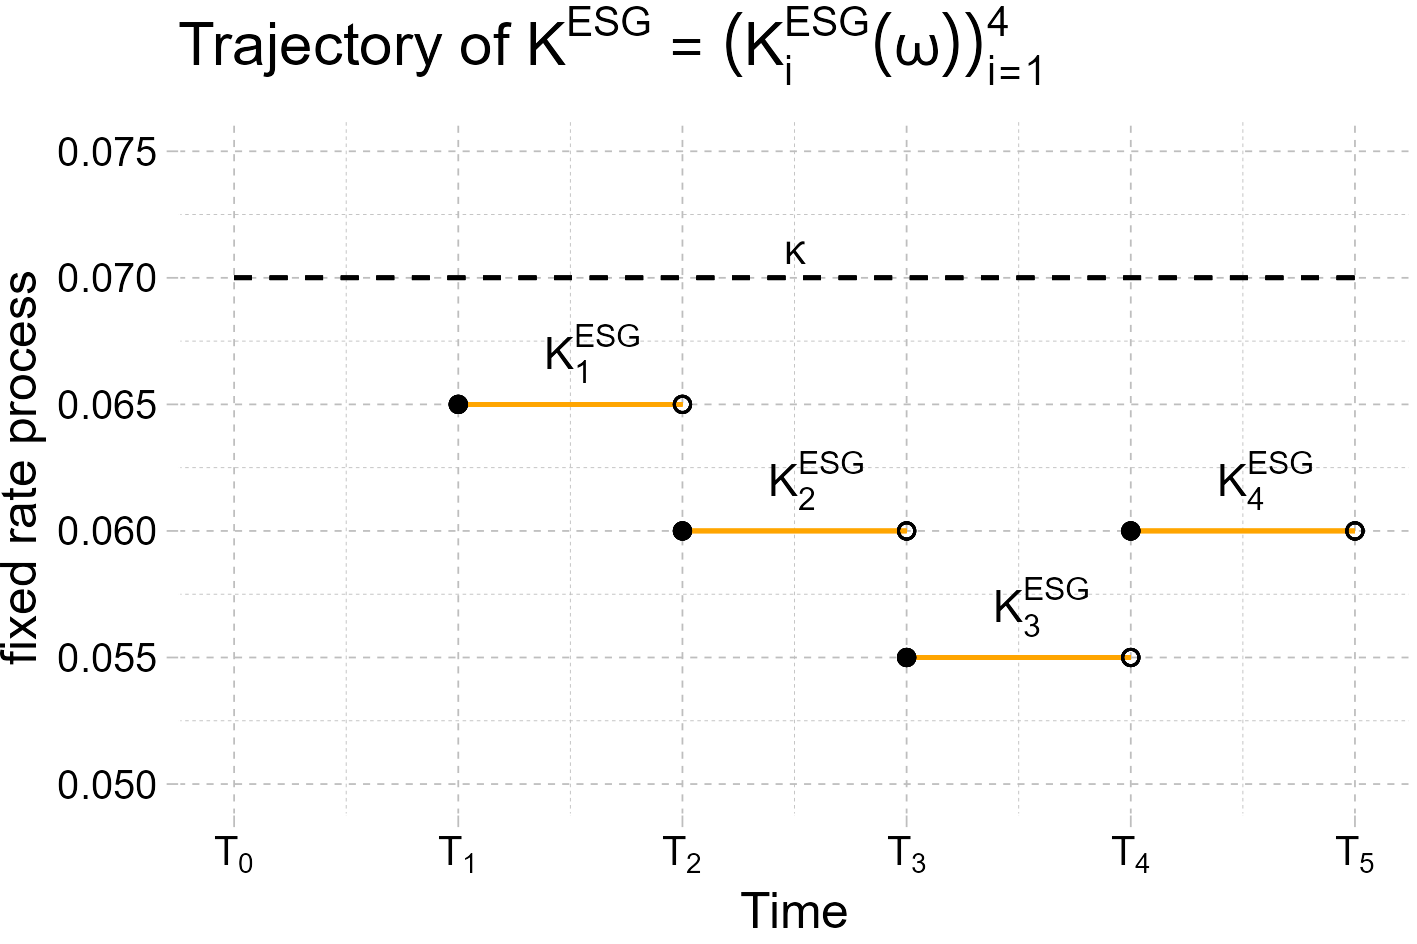
\includegraphics[width=10cm]{ESG/SBM_ESG_path.png}
    \caption{ESG-fixed rate trajectory}
    \label{fig: SBM_ESG_path}
\end{figure}
\end{frame}


\begin{frame}{ESG fixed rate}
\begin{notation}
Let $\mathcal{I} = \{k_{1}, \dots, k_{n}\}$ represent an index set. Let $\mathcal{H} 
\subseteq \mathcal{I}$, we then define: 
\begin{align*}
\left(
\bigcap_{i\in \mathcal{I}}A_{i}
\right)^{\mathcal{H}}
:= 
\left(
\bigcap_{i\in \mathcal{H}}A_{i}^{C}
\right)
\cap 
\left(
\bigcap_{i \in \mathcal{I}\setminus \mathcal{H}}A_{i}
\right)
\end{align*}
\end{notation}

\begin{example}
$\mathcal{I} = \{1,2,3,4,5\}$ and $\mathcal{H} = \{1,3,4\}$, this gives us: 

\begin{align*}
\left(
\bigcap_{i=1}^{5}A_{i}
\right)^{
\{1,3,4\}
}
&= 
A_{1}^{C}\cap A_{2}\cap A_{3}^{C}\cap A_{4}^{C}\cap A_{5}
\end{align*}    
\end{example}
\end{frame}


\begin{frame}{ESG fixed rate}
\begin{itemize}
    \item Let $n\in \mathbb{N}$, $\mathcal{I}_{n} := \{1, \dots, n\}$, $\mathcal{I}_{2n}^{Even} := \{2, \dots, 2n\}$
    \item $(A_{i})_{i \in \mathcal{I}_{n}}$ sequence of events measuring whether or not ESG-criteria is met:
    \[
    A_{i} = \{X_{T_{i}} \leq C_{T_{i}}^{ESG}\}
    \]
    \item ESG fixed rate process: $K^{ESG} = (K_{r}^{ESG}(\omega))_{r\in \mathcal{I}_{n}}$ 
\end{itemize}

\begin{observation}[Explicit form]
\begin{align*}
&K_{r}^{ESG}(\omega) = 
[\kappa -d\cdot r]\mathbbm{1}\left[
\bigcap_{i\in \mathcal{I}_{r}}A_{i}
\right](\omega)\; +\\ 
&\sum_{\alpha \in \mathcal{I}_{2r}^{Even}}
\left(
[\kappa -d\cdot (r-\alpha)]\mathbbm{1}\left[
\bigcup_{
j_{1}\neq \dots \neq j_{|\mathcal{I}_{\alpha}^{Even}|}
\in \mathcal{I}_{r}
}\left(
\bigcap_{i\in \mathcal{I}_{r}}A_{i}
\right)^{
\{
(j_{1}, \dots , j_{|\mathcal{I}_{\alpha}^{Even}|})
\}
}
\right]
\right)(\omega) 
\end{align*} 
\end{observation}
\end{frame}


\begin{frame}{ESG swap-rate process}
\begin{proposition}[Swap rate process $\kappa_{t}^{ESG} = (\kappa_{t}^{ESG}(i))_{i\in \mathcal{I}_{n}}$]
Denote $\kappa_{t}^{ESG}(i) := \E_{Q}[K_{i}^{ESG}(\omega)|\F_{t}]$. 
Then for $(t\leq T_{0})$ we have: 
\begin{align*}
\kappa_{t}^{ESG}(i)
&= 
\kappa -d\cdot D(i)
\end{align*}

Where: 
\begin{align*}
 D(i) &= 
i\cdot \E_{Q}\left[
\prod_{l=1}^{i}\mathbbm{1}(A_{l})\bigg{|}\F_{t}
\right] \\
&+ 
\sum_{\alpha \in \mathcal{I}_{2i}^{Even}}[i-\alpha]
\sum_{
j_{1}\neq \dots \neq j_{|\mathcal{I}_{\alpha}^{Even}|}
\in \mathcal{I}_{i}
}
\E_{Q}\left[
\left(
\prod_{l=1}^{i}\mathbbm{1}(A_{l})
\right)^{
\{
(j_{1}, \dots , j_{|\mathcal{I}_{\alpha}^{Even}|})
\}
}
\bigg{|}\F_{t}
\right]   
\end{align*}
\end{proposition}
\end{frame}



\subsection{Numerical Simulation}
\begin{frame}{Numerical Simulation}
\begin{itemize}
    \item $X(t)$: process representing the ESG-risk score in ESG-linked IRS. Proposal: 
    \begin{align*}
    X(t) &= 100\exp(-Z(t)) \\
    dZ(t) &= -\beta Z(t)dt + \sigma dW^{Q}(t) + dI^{Q}(t)
    \end{align*}
    \item $I^{Q}(t)$ is a CPP:
    \begin{align*}
    I^{Q}(t) &= \sum_{k=1}^{N(t)}J_{k}, \;\; J_{k}\sim  Exp(\mu),\;\; N(t) \sim Pois(\lambda t)    
\end{align*} 
\end{itemize}   
\end{frame}


\begin{frame}{Numerical Simulation}
\begin{figure}[htp]
    \centering
    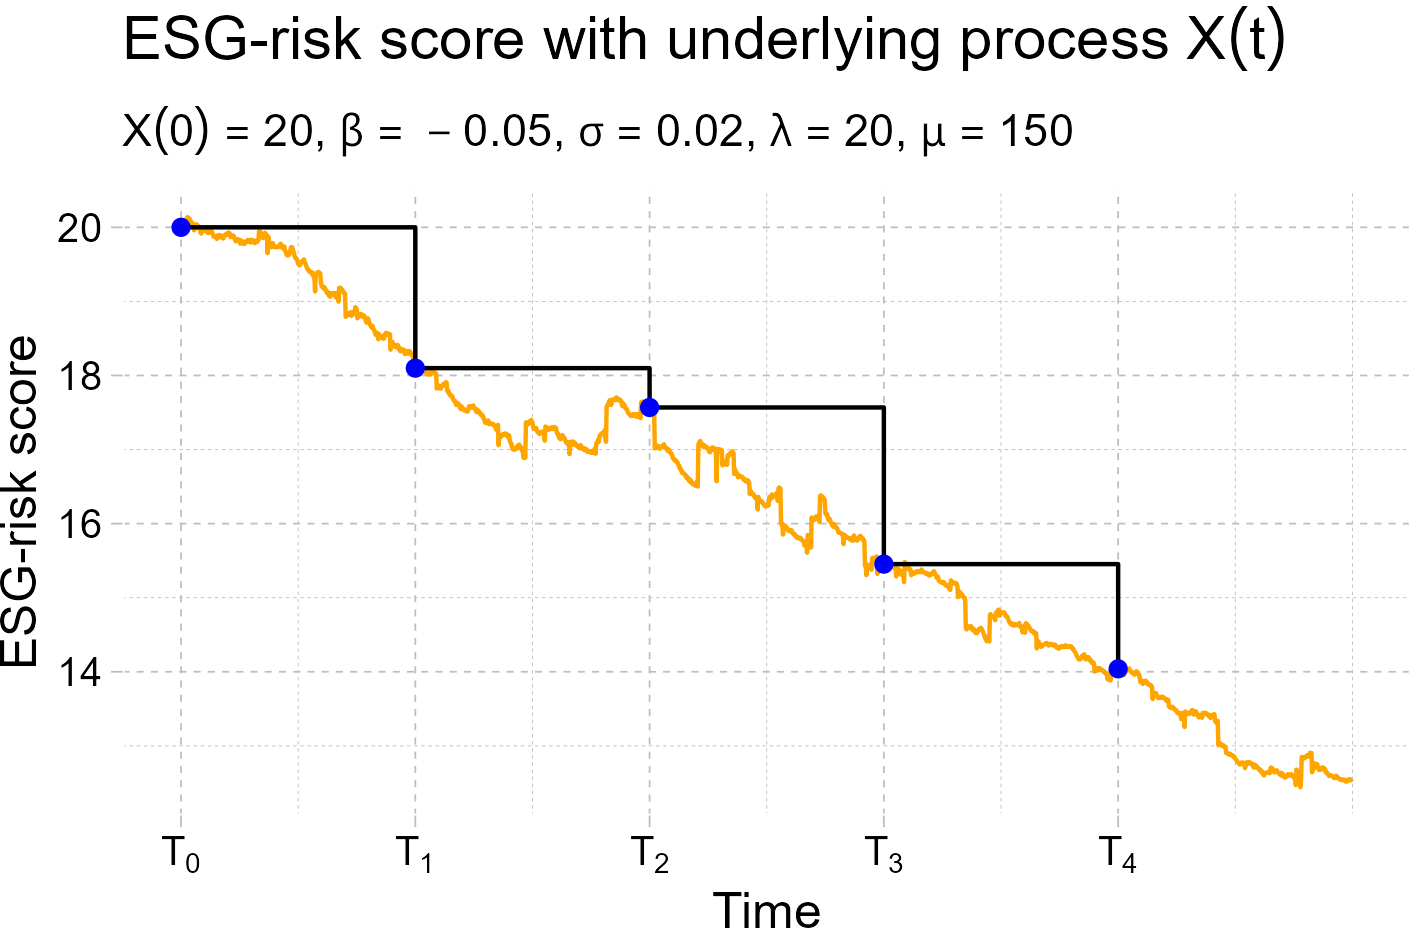
\includegraphics[width=10cm]{ESG/ESG_OU_path.png}
    \caption{ESG-risk score with underlying process $X(t)$}
    \label{fig: ESG_risk_score_underlying_X(t)}
\end{figure}
\end{frame}


\begin{frame}{Specifications}
\begin{itemize}
    \item $C^{ESG} = (C_{T_{i}}^{ESG})_{i\in \mathcal{I}_{4}}$, $\F_{0}$-measurable. 
    \item $\kappa_{t}^{ZCB} = 0.07$, the fixed-rate from the original IRS. 
    \item $d = 0.005$ constant penalty/discount. 
    \item $\delta:= T_{i}-T_{i-1} = 1$ 
\end{itemize}
We will showcase some scenarios where we consider "reasonable" and "unreasonable" ESG-criteria $C_{T_{i}}^{ESG}$. 

\end{frame}

\begin{frame}{Reasonable criteria}
\begin{itemize}
    \item $C^{ESG} = (17.8, 16.8, 15.8, 14.8)$
\end{itemize}
\begin{figure}[htp]
    \centering
    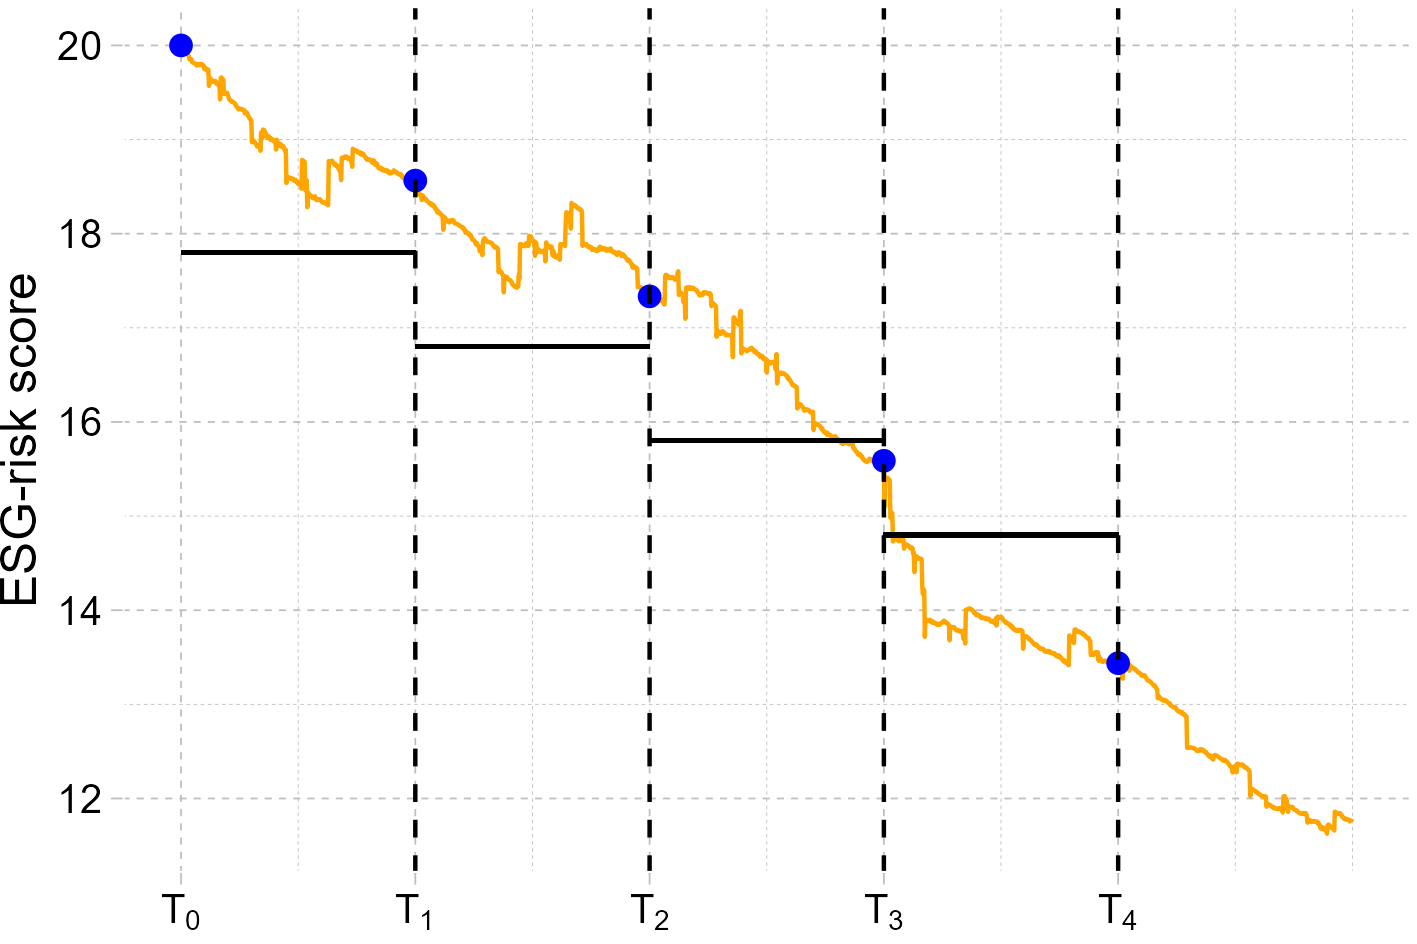
\includegraphics[width= 8cm]{ESG/ESG_plt_criteria1.png}
    \caption{ESG-risk score where ESG-criteria is reasonable}
    \label{fig: ESG_risk_criteria1}
\end{figure}    
\end{frame}


\begin{frame}{Reasonable criteria}
\begin{figure}[htp]
    \centering
    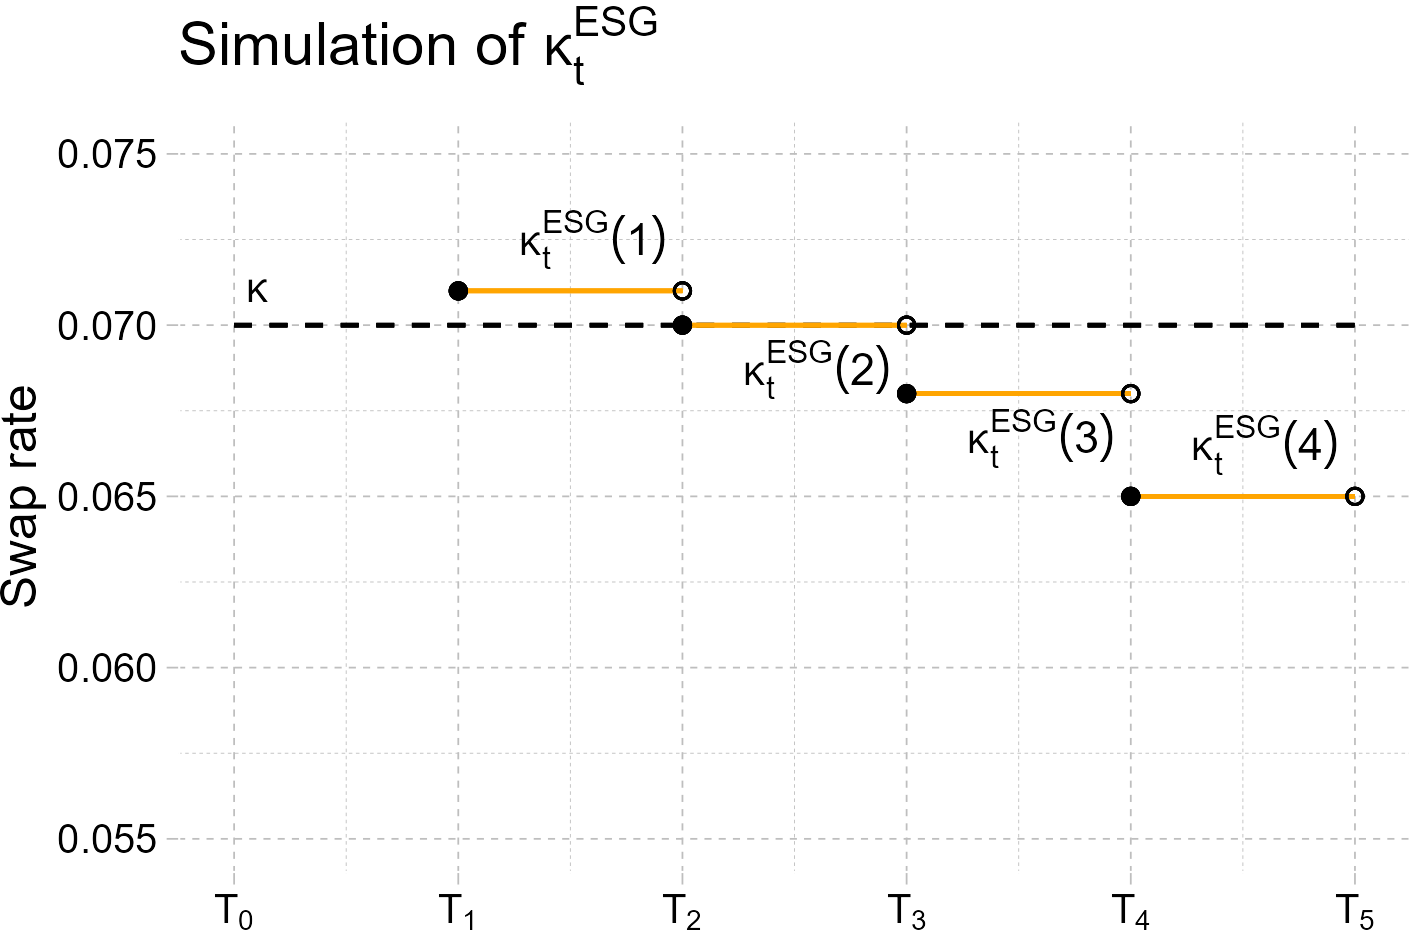
\includegraphics[width= 9cm]{ESG/kappa_t_ESG_1.png}
    \caption{ESG-swap rate when ESG-criteria is reasonable}
    \label{fig: ESG_swap_1}
\end{figure}
\end{frame}



\begin{frame}{Unreasonable Criteria}
Always managing to meet criteria: 
$C^{ESG} = (24,23,22,21)$
\begin{figure}[htp]
    \centering
    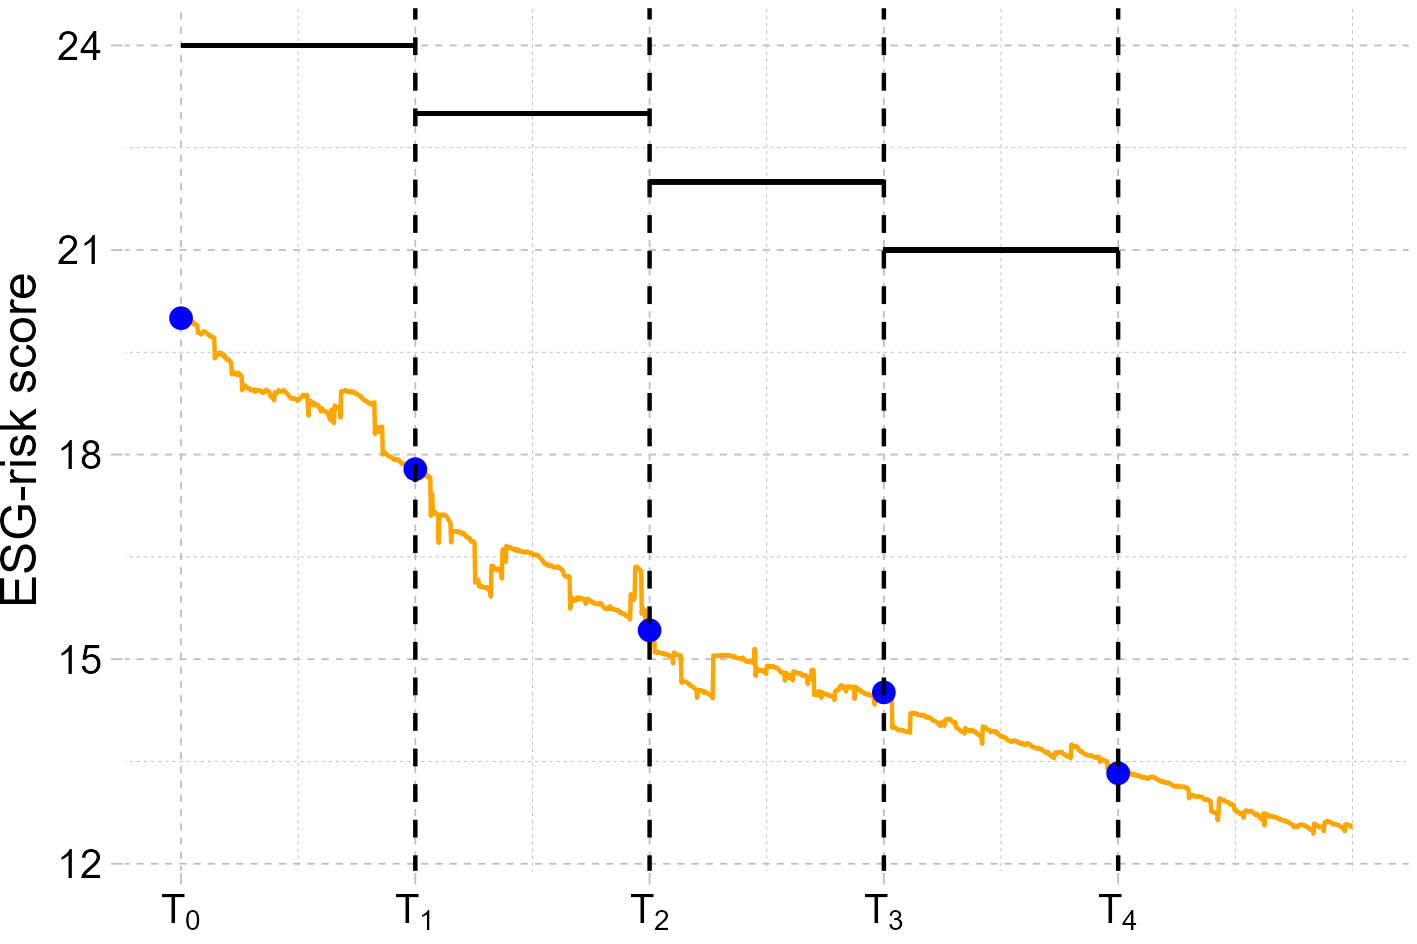
\includegraphics[width= 9cm]{ESG/ESG_plt_criteria2.png}
    \caption{ESG-risk score where ESG-criteria is always met}
    \label{fig: ESG_risk_criteria_2}
\end{figure}
\end{frame}

\begin{frame}{Unreasonable Criteria}
\begin{figure}[htp]
    \centering
    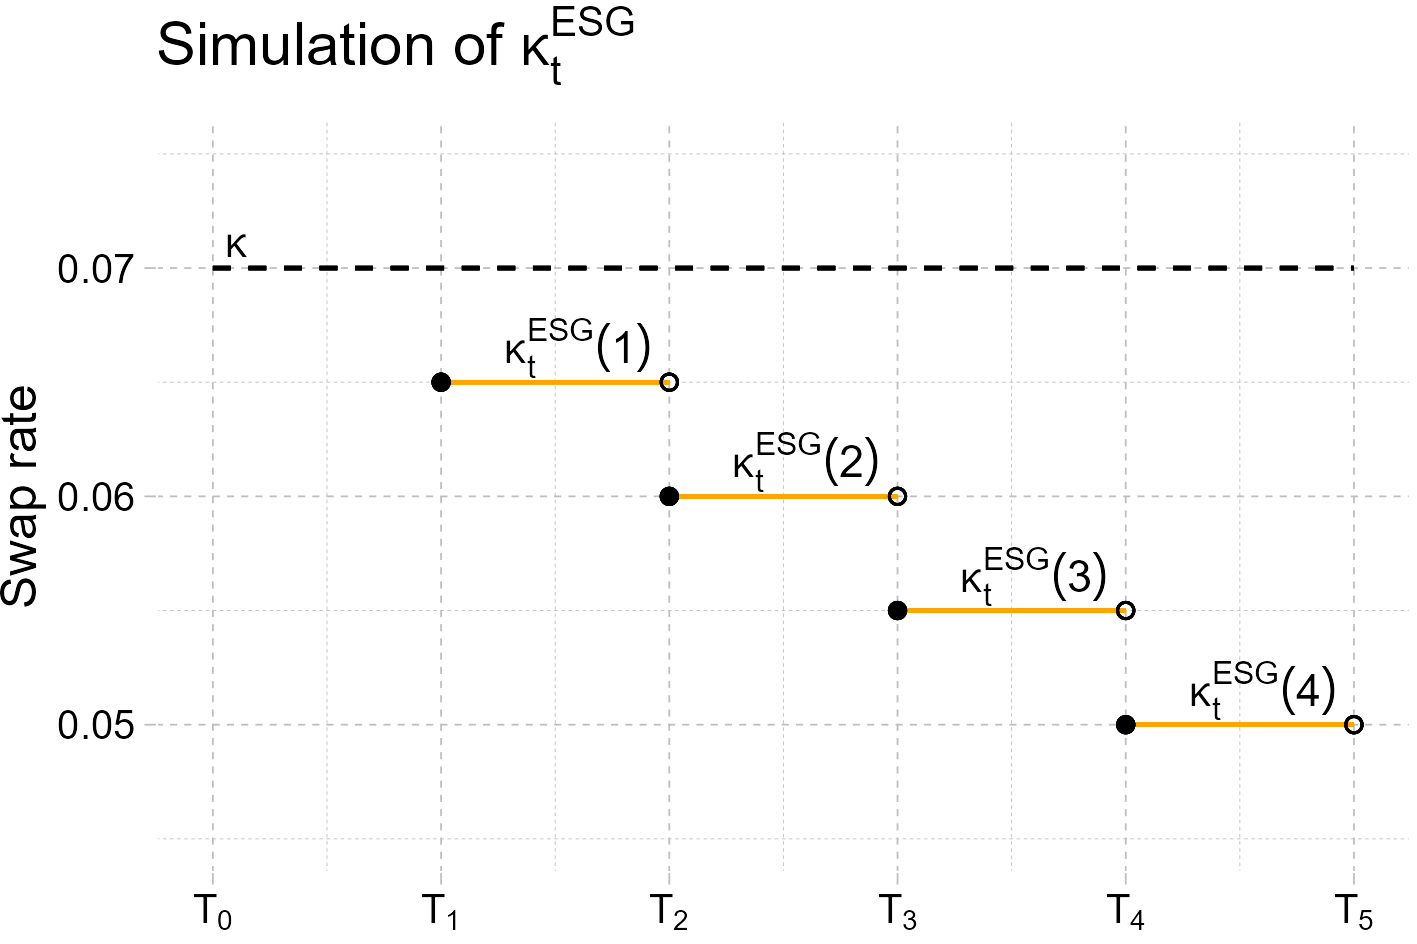
\includegraphics[width= 9cm]{ESG/kappa_t_ESG_2.png}
    \caption{ESG-swap rate, when ESG-criteria is always met}
    \label{fig: ESG_swap_2}
\end{figure}
\end{frame}


\section{Conclusions and further work}
\SectionPage

\subsection{SOFR: Conclusion and further work}
\begin{frame}{SOFR: Conclusion and further work}
\begin{itemize}
    \item SOFR: overnight, thus 1-tenor: 24h. 
    \item futures market: market view on future rates. 
    \item CME term-SOFR: inferred from the futures market. 
    \item Further work: look more into the modelling of term-SOFR, closely related to EFFR (Effective Federal Funds Rate), as discussed in: \cite{gellert2021short}.  
    \item Hedge: we used a one-factor model and operated under $Q$. More reasonable: multi-factor models and suitable $ P$ dynamics. Following the author's approach in \cite{SS20} 
\end{itemize}
\end{frame}

\subsection{ESG: Conclusion and further work}
\begin{frame}{ESG: Conclusion and further work}
\begin{itemize}
    \item ESG-criteria: 
    \[
    A_{i} = \{X_{T_{i}} \leq C_{T_{i}}^{ESG}\}
    \]
    \item $C^{ESG}$: $\F_{T_{i-1}}$-measurable instead of $\F_{0}$. 
    \item Choice of process $X = (X(t))_{t\in[0,T]}$ important. Which one to choose? 
    \item ESG-score/risk-score will be observed under $P$, not $Q$. Complex transformations. 
    \item Data accessibility, standardization of score $\mathcal{S}$: 
    \begin{align*}
     \mathcal{S} := \sum_{j=1}^{m}w_{j}X_{j}   
    \end{align*}
    \item how to choose the weights $w_{j}$'s and which metrics to $X_{j}$'s should one choose?
    Different agencies can give different scores to the same company, further discussed in \cite{Billio2021}.  
\end{itemize}
\end{frame}


\begin{frame}{ESG: Conclusion and further work}
\begin{itemize}
    \item Closed expression for $K_{n}^{ESG}(\omega)$, quite complex, requires the Monte-Carlo approach. However, it gives flexibility for modelling ESG scores/risk scores. 
\end{itemize}
\end{frame}



\begin{comment}
\begin{frame}{Framework}
    \begin{theorem}[Fermat's little theorem]
        For a prime~\(p\) and \(a \in \mathbb{Z}\) it holds that \(a^p \equiv a \pmod{p}\).
    \end{theorem}
    
    \begin{proof}
        The invertible elements in a field form a group under multiplication.
        In particular, the elements
        \begin{equation*}
            1, 2, \ldots, p - 1 \in \mathbb{Z}_p
        \end{equation*}
        form a group under multiplication modulo~\(p\).
        This is a group of order \(p - 1\).
        For \(a \in \mathbb{Z}_p\) and \(a \neq 0\) we thus get \(a^{p-1} = 1 \in \mathbb{Z}_p\).
        The claim follows.
    \end{proof}

\end{frame}
\end{comment}




\section{References}


\begin{frame}[allowframebreaks]{References}
    \begin{thebibliography}{}

        % Article is the default.
        \setbeamertemplate{bibliography item}[book]
        
        
        %\bibitem{Hartshorne1977}
        %Hartshorne, R.
        %\newblock \emph{Algebraic Geometry}.
        %\newblock Springer-Verlag, 1977.

        \setbeamertemplate{bibliography item}[article]

        
        %\bibitem{Helso2020}
        %Helsø, M.
        %\newblock \enquote{Rational quartic symmetroids}.
        %\newblock \emph{Adv. Geom.}, 20(1):71--89, 2020.

        \setbeamertemplate{bibliography item}[online]

        \bibitem{ISDA_2021}
        ISDA, 2021 
        \newblock \enquote{Overview of ESG-related derivatives products and transactions}
        \newblock \url{https://www.isda.org/a/qRpTE/Overview-of-ESG-related-Derivatives-Products-and-Transactions.pdf}
        

        %\bibitem{SS20}
        %Skov, J. B. and Skovmand, D
        %\newblock \enquote{Dynamic term structure models for SOFR futures, 2020} 
        %\newblock
        %\url{https://papers.ssrn.com/sol3/papers.cfm?abstract_id=3692283}
        

        %\bibitem{HR2018}
        %Helsø, M.\ and Ranestad, K.
        %\newblock \emph{Rational quartic spectrahedra}, 2018.
        %\newblock \url{https://arxiv.org/abs/1810.11235}

        \setbeamertemplate{bibliography item}[triangle]

        %\bibitem{AM1969}
        %Atiyah, M.\ and Macdonald, I.
        %\newblock \emph{Introduction to commutative algebra}.
        %\newblock Addison-Wesley Publishing Co., Reading, Mass.-London-Don
        %Mills, Ont., 1969

        \setbeamertemplate{bibliography item}[text]

        

        \bibitem{SS20}
        Skov, J. B. and Skovmand, D
        \newblock \enquote{Dynamic term structure models for SOFR futures, 2020} 
        \newblock
        \url{https://papers.ssrn.com/sol3/papers.cfm?abstract_id=3692283}

        \bibitem{gellert2021short}
        Gellert, Karol and Schloegl, Erik
        \newblock \enquote{Short Rate Dynamics: A Fed Funds and SOFR perspective, 2021}
        \newblock 
        \url{https://ssrn.com/abstract=3763589}

        \bibitem{Billio2021}
        Billio, Monica et al. 
        \newblock \enquote{Inside the ESG ratings: (Dis)agreement and performance, 2021}
        \newblock \url{https://onlinelibrary.wiley.com/doi/abs/10.1002/csr.2177}
        
        

        %\bibitem{Artin1966}
        %Artin, M.
        %\newblock \enquote{On isolated rational singularities of surfaces}.
        %\newblock \emph{Amer. J. Math.}, 80(1):129--136, 1966.

    \end{thebibliography}
\end{frame}


\begin{comment}
@article{Billio2021,
author = 
{Billio, Monica and Costola, Michele and Hristova, Iva and Latino, Carmelo and Pelizzon, Loriana
},
title = {
Inside the ESG ratings: (Dis)agreement and performance
},
journal = {
Corporate Social Responsibility and Environmental Management
},
volume = {28},
number = {5},
pages = {1426-1445},
keywords = {Corporate Social Responsibility, ESG rating agencies, sustainable investments},
doi = {https://doi.org/10.1002/csr.2177},
url = {https://onlinelibrary.wiley.com/doi/abs/10.1002/csr.2177},
eprint = {https://onlinelibrary.wiley.com/doi/pdf/10.1002/csr.2177},
year = {2021}
}    
\end{comment}

\end{document}